\chapter{Ejercicios resueltos}

%%%%%%%%%%%%%%%%%%%%%%%%%%%%%%%%%%%%%%%%%%%%%%%%%%

\emph{Este capítulo se basa en los ejemplos. Se propondrán una serie
de ejercicios, se comentarán los algoritmos necesarios para resolverlos
y finalmente se dará la solución a cada uno de ellos. }


\section*{Metodología de programación}

Quizás el mayor punto fuerte de Matlab o Octave no es su sencillez o
su productividad sino la gran cantidad de funciones útiles que nos
proporcionan. El núcleo de Matlab son sólo unos pocos Mbytes, en
cambio la instalación completa ocupa tres CD-ROMs. Todo son funciones
y archivos cuya razón de ser es hacernos la vida mucho más fácil.

Esto genera una ley un poco paradójica: \textbf{cuanto menos
  programemos mejores serán nuestros scripts}. Uno puede pensar que el
código que escribe uno mismo es mejor, que si al intuitérprete le pasamos
todas las líneas que debe usar irá más rápido. Que si tenemos que
cargar más funciones en memoria haremos que la ejecución vaya más
lenta...  Es justo lo contrario. La mayoría de las funciones en
Octave, por ejemplo, son funciones escritas en C++ o en Fortran
compiladas de una manera especial para que Octave las interprete.
Significa que la velocidad de ejecución de estas subrutinas será mucho
más cercana a la velocidad de los programas binarios que a la del
intérprete.


\section{Ejercicio. Cálculo de un gradiente}

Un cálculo muy común con una muestra de datos bidimensional es
calcular una especie de gradiente numérico definido como:$$
grad(M)=\left(\begin{array}{c}
    \frac{M(i,j+1)-M(i,j-1)}{2}\\
    \frac{M(i+1,j)-M(i-1,j)}{2}\end{array}\right)=\left(\begin{array}{c}
    \delta_{x}^{\prime}(M)\\
    \delta_{y}^{\prime}(M)\end{array}\right)$$ Que genera una matriz
de menor tamaño al perder los extremos. Escribir la función que
devuelve el resultado en una variable tipo estructura:
\texttt{grad.x}=$\delta_{x}^{\prime}(M)$ y
\texttt{grad.y}=$\delta_{y}^{\prime}(M)$.


\subsection{Guía para la resolución del ejercicio}

Lo más complicado de este ejercicio es entender el enunciado. En el
fondo es exactamente el mismo cálculo que un gradiente numérico con
la diferencia de que en este caso no nos importa la distancia entre
los puntos. Lo más práctico para calcular la fórmula es construir
una submatriz por cada elemento de la ecuación en diferencias; para
calcular la submatriz es necesario saber que el último elemento de
cualquier matriz o vector se puede llamar \texttt{end}. Por ejemplo,
si nosotros queremos los elementos del quinto al último del vector
\texttt{u} pero no sabemos sus dimensiones, en vez de calcularlo lo
más práctico es hacer \texttt{>\,{}> u(5:end)}.


\subsection{Solución del ejercicio}

  \begin{verbatim}
function[grad]=mygradient(M)

    grad.x = 0.5*(M(:,3:end)-M(:,1:end-2));

    grad.y = 0.5*(M(3:end,:)-M(1:end-2,:));
 \end{verbatim}


\section{Ejercicio.  Diseño de una tobera}

Queremos diseñar una tobera convergente divergente. Para ello
impondremos que el radio de salida sea 10 veces mayor que el radio de
la garganta, y que la tobera se forma mediante dos parábolas, una con
eje en $y$ y otra con eje en $x$. Las condiciones serán que en el
punto de empalme de los dos arcos haya continuidad tanto de la función
como de la derivada primera. Las dos funciones a ajustar serán
entonces (con el problema
convenientemente adimensionalizado)\\
$$y^{-}=Px^2+0.1\qquad y^{+}=\sqrt{Ax+B}$$
Entonces tenemos el sistema de ecuaciones siguiente, donde $l$ es el
punto en $x$ donde se empalman los dos arcos:
$$2Pl=\frac{A}{2\sqrt{Al+B}}$$
$$Pl^2+0.1=\sqrt{Ax+B}$$
$$\sqrt{A+B}=1$$
Donde se demuestra que existe solución para $P$ aproximadamente
$0.9<P<1.2$.

\begin{enumerate}
\item Resolver el sistema de ecuaciones anterior y representar las
  soluciones de $P=0.9$, $P=1$ y $P=1.2$
\end{enumerate}

\subsection{Guía para la resolución del ejercicio}

Lo primero que debemos hacer es entender el enunciado, para ver más
claro lo que se pide, es bueno dibujar las dos curvas que se nos proponen,
para ello haremos;

\begin{verbatim}
octave:1> fplot('[x. ^2+0.1,sqrt(x)]',[0,1])
\end{verbatim}
Para resolver numéricamente sistemas de ecuaciones lineales usaremos
la función \texttt{fsolve}. Para saber cómo funciona teclearemos en
la línea de comandos: 

\begin{verbatim}
octave:2> help fsolve
\end{verbatim}

\subsection{Solución del ejercicio}

El script que nos resuelve el problema es el siguiente: 

\begin{verbatim}
function[f]=ttb(x)
    global Pi
    f(1)=x(1)/(2*sqrt(x(1)*x(3)+x(2)))-2*Pi*x(3);
    f(2)=Pi*x(3)**2+0.1-sqrt(x(1)*x(3)+x(2));
    f(3)=sqrt(x(1)+x(2))-1;
end   
  
function[f]=tobera(x,a,b,l,P)
    if x<l
      f=P*(x*x)+0.1;
    else
      f=sqrt(a*x+b);
    endif
end   
x0=[1 1 1];
P=[0.9 1 1.2];
hold on   
for i=1:3
  global Pi
  Pi=P(i);
  [res]=fsolve('ttb',x0);
  xcoord=linspace(0,1,100);   
  for j=1:100
    tob(j)=tobera(xcoord(j),res(1),res(2),res(3),P(i));
  end
  plot(xcoord,tob)
end   
   
hold off
\end{verbatim}

El resultado lo vemos en la figura \ref{cap:Resultado-del-script-53}.

%
\begin{figure}[H]
\centering{}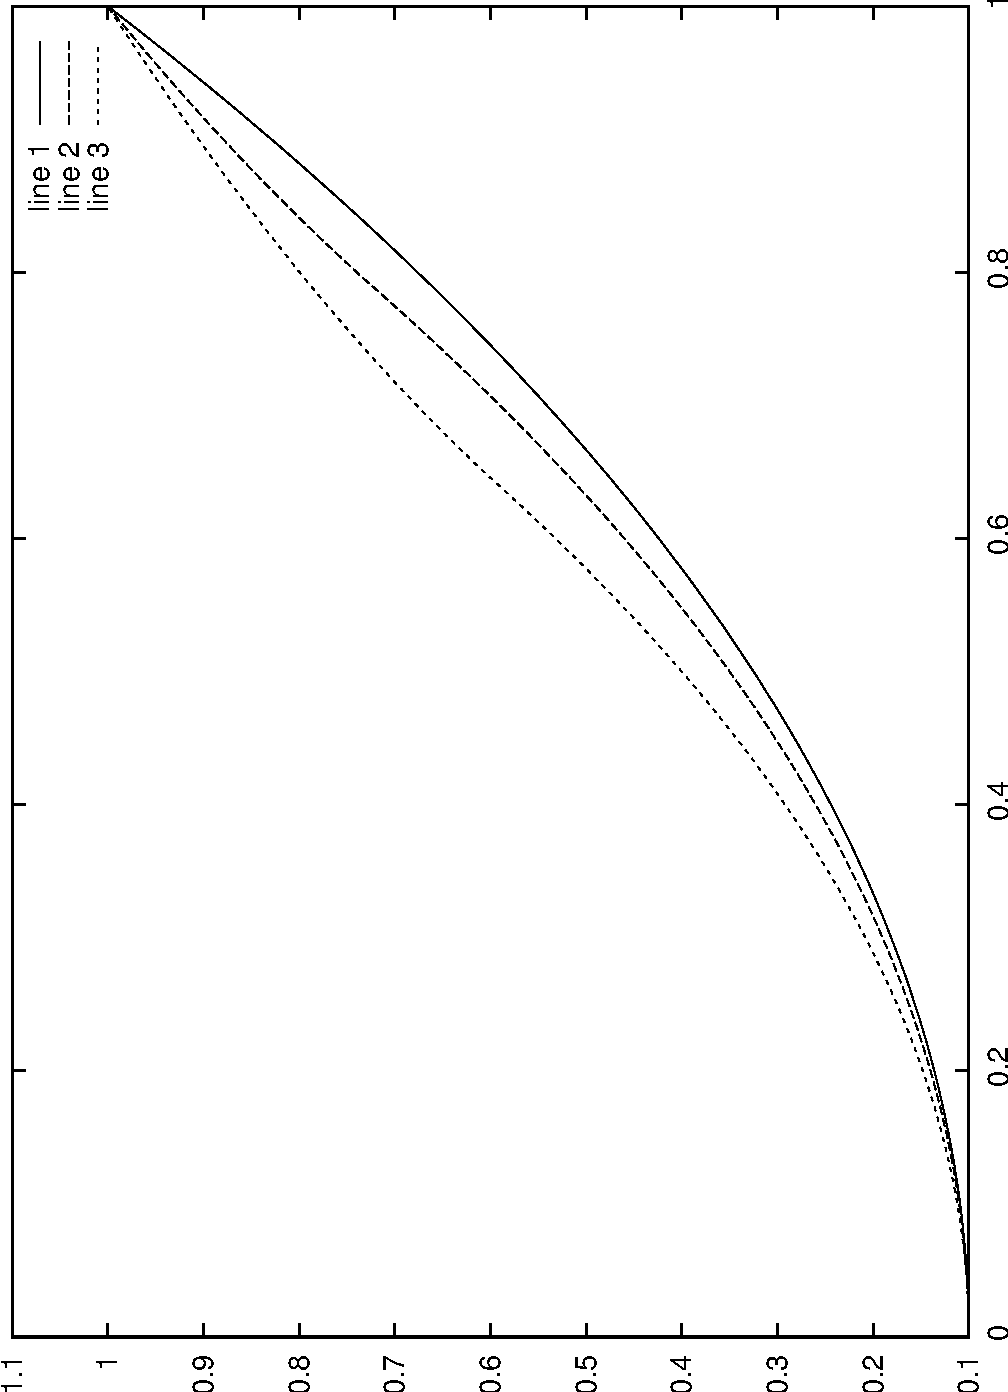
\includegraphics[%
  width=8cm,
  keepaspectratio,
  angle=-90]{figuras/figuraejercicio2}


\caption{\label{cap:Resultado-del-script-53}Resultado del script}
\end{figure}



\section{Ejercicio\label{sec:Ejercicio ode}.  El atractor de Lorentz}

Se quiere integrar la ecuación diferencial del \emph{Atractor de
  Lorentz}\index{Lorentz}, de ecuaciones:
$$
\begin{array}{l}
  \dot{x}=a(y-x)\\
  \dot{y}=x(b-z)-y\\
  \dot{z}=xy-cz\end{array}\qquad con\qquad a=10,\,\, b=28,\,\, c=\frac{8}{3}$$
y representarla en el espacio.


 \subsection{Guía para la resolución del Ejercicio}

 \begin{itemize}
 \item Primero escribimos la función correspondiente a la ecuación
   diferencial.  En las subrutinas de resolución de EDOs siempre
   tenemos que introducir la función de la forma
   $\frac{dx}{dt}=f(x,t)$ pudiendo ser cualquiera de las variables un
   vector.
 \item La rutina de Octave que nos integra la ecuación diferencial es
   \texttt{lsode}; en Matlab utilizaremos \texttt{ode45} porque el
   problema no es stiff.  Utilizar la ayuda para saber de qué manera
   tenemos que escribir la función de la ecuación diferencial.
 \item El comando para representar curvas paramétricas en 3
   dimensiones es \texttt{plot3}.
 \item Escribiremos todo en un script y lo ejecutaremos
 \end{itemize}

\subsection{Solución del ejercicio}


\subsubsection{Octave}

\begin{verbatim}
x=0;
function xdot=func(x,t)
a=10;b=28;c=8/3;
xdot(1,1)=a*(x(2)-x(1));
xdot(2,1)=x(1)*(b-x(3))-x(2);
xdot(3,1)=x(1)*x(2)-c*x(3);
end

x0=[1;1;1];
t=linspace(0,50,5000);
tic;x=lsode( "func ",x0,t);toc
plot3(x(:,1),x(:,2),x(:,3))
\end{verbatim}
dando como resultado la figura \ref{cap:Resultado-del-script-54}:

%
\begin{figure}[h]
\centering{}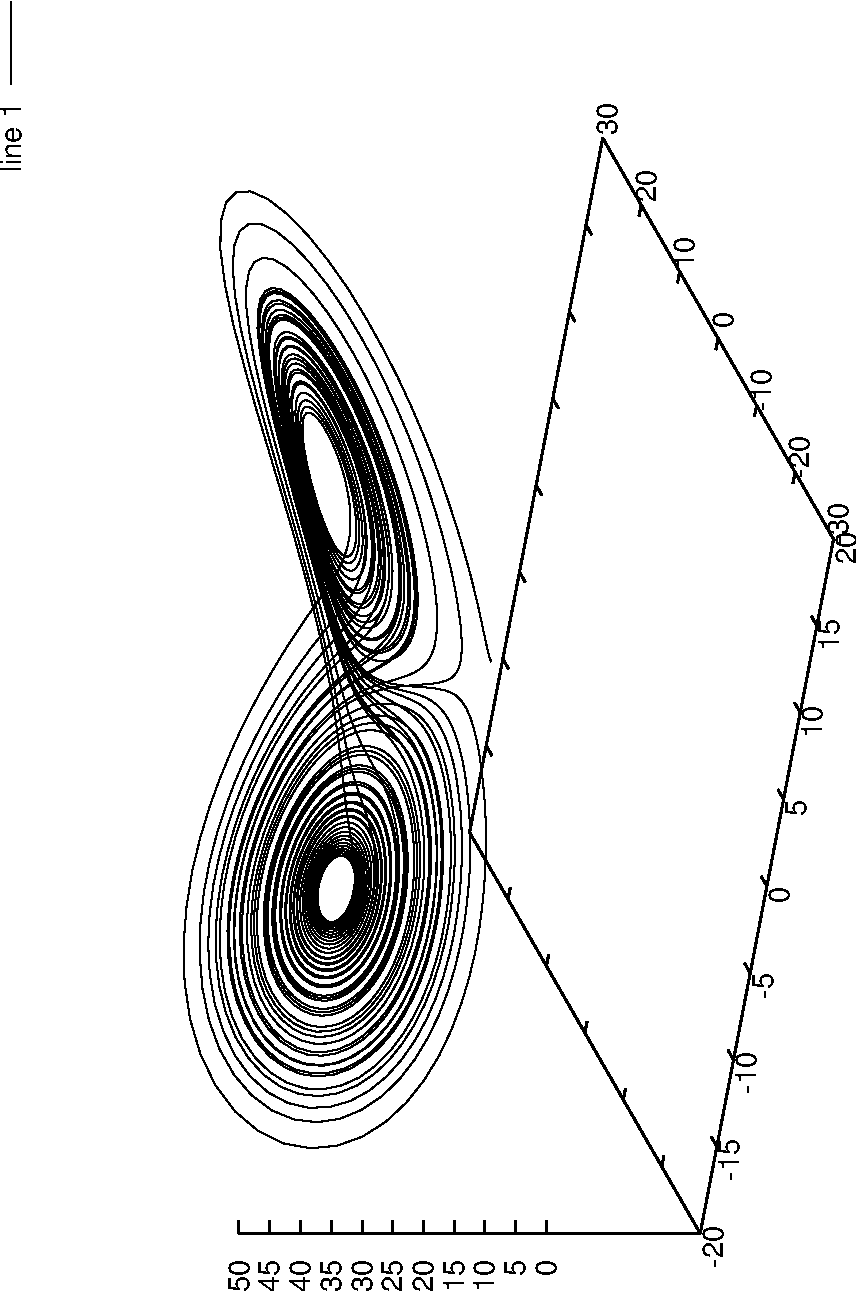
\includegraphics[%
  width=9cm,
  keepaspectratio,
  angle=-90]{figuras/figuraejercicio3}


\caption{\label{cap:Resultado-del-script-54}Resultado del script}
\end{figure}
 y el tiempo necesario para resolver la EDO que es de $3.1488$ segundos

La función \texttt{lsode} es mucho más versátil que las funciones
para la integración de ecuaciones diferenciales de Matlab. También
lo es en el sentido que es menos rigurosa en la manera de escribir
la función, en este caso hemos escrito la variable \texttt{xdot} en
forma de vector columna como nos obliga Matlab pero aceptaría igualmente
el uso de un vector columna.

Octave permite definir la función en el script de modo que podemos
resolver el problema con un único archivo.


\subsubsection{Octave no stiff}

El método de integración por defecto es explícito de modo que podemos
acelerar el proceso si utilizamos un esquema Adams-Bashforth incluyendo
este comando en el script:

\begin{verbatim}
lsode_options('integration method','non-stiff')
\end{verbatim}
Podemos hacerlo sin miedo porque el problema del atractor de Lorentz,
aunque es caótico, no es stiff. El tiempo de ejecución desciende a
$2.0016$ segundos.


\subsubsection{Octave y C++}

Ya hemos visto que podemos utilizar funciones escritas en otros
lenguajes para aumentar la velocidad de nuestros scripts. En el caso
de este ejercicio la velocidad conseguida por la función
\texttt{lsode} es aceptable pero podemos rebajarla bastante más
escribiendo la función de la ecuación diferencial en C++ y utilizando
la aplicación \texttt{mkoctfile}.  Ya hemos aprendido a hacerlo en la
sección \ref{sec:Extender-Octave-con}.  Supongamos que ya disponemos
del archivo \texttt{eqlorentz.oct} que usaremos del mismo modo que
cualquier función. El script que resuelve el problema es:

\begin{verbatim}
t=linspace(0,50,5000);
tic;x=lsode( "eqlorentz ",[1;1;1],t);toc
plot3(x(:,1),x(:,2),x(:,3))
\end{verbatim}

La nueva versión del script es capaz de resolver el problema en tan
sólo $0.28444$ segundos que es el 10\% del tiempo anterior.


\subsubsection{Octave y C++ no stiff}

La máxima optimización se consigue de este modo. El tiempo se rebaja
hasta $0.17314$ segundos. Aunque todas estas consideraciones sobre
velocidad pueden parecer inútiles debemos tener en cuenta que la
integración de EDOs y EDPs son los problemas numéricos más exigentes
en lo que respecta a uso de CPU. Entrar en este tipo de discusiones a
menudo comporta grandes beneficios aunque en este caso sean
irrisorios. Este último tiempo es comparable al obtenido con código
enteramente escrito en C++ y sólo un poco más lento que el escrito en
C o Fortran y el esfuerzo necesario para escribir el programa ha sido
mucho menor.%
\footnote{El uso de lenguajes {}``pegamento'' es una práctica cada día
  más habitual. Escribir un código enteramente en C o Fortran es
  bastante costoso tanto por el tiempo de desarrollo como por el
  esfuerzo necesario.  Muchas veces se empieza con un prototipo
  escrito con un lenguaje de RAD (Rapid Application Development) y
  posteriormente se reescriben sus partes.

  El mayor obstáculo en los proyectos grandes es que deben participar
  varios desarrolladores. Cada uno puede tener sus preferencias y las
  guías de estilo no siempre son una solución efectiva porque sólo
  arreglan el formato del código escrito. Todas estas dificultades
  unidas al aumento de velocidad de lenguajes como Python o Matlab ha
  llevado a la creación del concepto de {}``lenguaje pegamento''.

  Se trata de dejar a medias el código entre el prototipo y el
  programa definitivo. Partiendo del prototipo se van analizando las
  partes que consumen más recursos y, sin cambiar las cabeceras ni el
  esquema de variables, se reescriben en algún lenguaje rápido. Se
  para cuando se consigue un equilibrio entre nivel de interactividad,
  velocidad y coste de mantenimiento de código.

  Probablemente el mejor {}``lenguaje pegamento'' sea Python gracias a
  Pyrex, SWIG y F2Py. El primero es capaz de convertir el código
  Python en C++ automáticamente (rendimiento máximo y coste cero) y el
  segudo y el tercero son generadores automáticos de interfaces, SWIG
  para C y C++ y F2Py para Fortran 77 y Fortran 95.%
}


\subsubsection{Octave, C++ y Fortran}

Fortran es el lenguaje del cálculo matricial por excelencia. Hemos
visto ya la manera de producir wrappers para funciones en Fortran.
Su utilidad, más que para escribir pequeñas funciones donde el wrapper
puede ser más largo que el código útil, es la de acoplar subrutinas
que hagan uso de grandes cantidades de memoria con distintas precisiones
en coma flotante. La velocidad de Fortran es aproximadamente la misma
que la de C++ pero aporta ventajas distintas a la velocidad por lo
dicho anteriormente.


\subsubsection{Matlab}

En Matlab necesitaremos dos archivos. El archivo de función devuelve
el resultado en forma de vector columna (\texttt{lorentz.m}):

  \begin{verbatim}
function xdot=lorentz(t,x)
  a=10;b=28;c=8/3;
  xdot(1,1)=a*(x(2)-x(1));
  xdot(2,1)=x(1)*(b-x(3))-x(2);
  xdot(3,1)=x(1)*x(2)-c*x(3);
end
 \end{verbatim}
Fijémonos que el orden de las variables de la cabecera \texttt{x}
y \texttt{t} cambian según la rutina que usemos. El script será:

  \begin{verbatim}
x=0;t=0;
tic;[t,x]=ode45(@lorentz,[0,50],[1,1,1]);toc
plot3(x(:,1),x(:,2),x(:,3))
 \end{verbatim}

\section{Ejercicio.  Cálculo de una integral doble}

La integral
$$I=\int_{-\infty}^{\infty}\int_{-\infty}^{\infty}e^{-(x^{2}+y^{2})}dx\  dy$$
tiene como resultado $\pi$. Calcular la solución \textbf{con un único
comando}.


\subsection{Guía para la resolución del ejercicio}

La función que implementa la integral doble en matlab es \texttt{dblquad}
mientras que en Octave es \texttt{quad2dg}. Ambas funciones tienen
una cabecera idéntica, las únicas diferencias son el nombre y el algoritmo
de cálculo. Para pasarles la función a integrar como argumento usaremos
una sentencia \texttt{inline} o con una función anónima. Las rutinas
de integración tienen muchos problemas con las singularidades porque
trabajan con una precisión limitada, esto nos impide usar límites
de integración demasiado grandes y ni mucho menos podremos usar \texttt{Inf}
. Con $[-10,10]\times[-10,10]$ vamos a conseguir 5 cifras significativas.

Por si alguien aún no está trabajando con Octave esta es la ayuda
de la función \texttt{quad2dg}.

  \begin{verbatim}


>> help quad2dg
quad2dg is the user-defined function from the file
/usr/share/octave/2.1.64/site/m/octave-forge/integration/quad2dg.m   
usage:  int = quad2dg('Fun',xlow,xhigh,ylow,yhigh)
or
       int = quad2dg('Fun',xlow,xhigh,ylow,yhigh,tol)   
This function is similar to QUAD or QUAD8 for 2-dimensional integration,
but it uses a Gaussian quadrature integration scheme.
      int     -{}- value of the integral
      Fun     -{}- Fun(x,y) (function to be integrated)
      xlow    -{}- lower x limit of integration
      xhigh   -{}- upper x limit of integration
      ylow    -{}- lower y limit of integration
      yhigh   -{}- upper y limit of integration
      tol     -{}- tolerance parameter (optional)   
  
Note that if there are discontinuities the region of integration
should be broken up into separate pieces.  And if there are singularities,
a more appropriate integration quadrature should be used
(such as the Gauss-Chebyshev for a specific type of singularity).
 \end{verbatim}

\subsection{Solución del ejercicio}

\begin{itemize}
\item Matlab:
\begin{verbatim}
>> dblquad(@(x,y) exp(-(x.^2+y.^2)),-10,10,-10,10)
ans = 3.1416
\end{verbatim}
\item Octave:
\begin{verbatim}
>> quad2dg(@(x,y) exp(-(x.^2+y.^2)),-10,10,-10,10)
ans = 3.1416
\end{verbatim}
\end{itemize}

\section{Ejercicio\label{sec:Ejercicio-Laplace}.  Resolución de la
  ecuación de Laplace en un dominio bidimensional}

Resolver la ecuación de Laplace en un dominio rectangular por
diferencias finitas con condiciones de contorno Dirichlet. La ecuación
de Laplace es la ecuación elíptica más sencilla: $\nabla^{2}\phi=0$,
que formulada en dos dimensiones se convierte en:\[
\frac{\partial^{2}\phi}{\partial
  x^{2}}+\frac{\partial^{2}\phi}{\partial y^{2}}=0\] Si se toman
diferencias finitas centradas de segundo orden para puntos dependiendo
de $i$ y $j$ llegamos a la ecuación en diferencias siguiente:

$$\frac{\phi(i+1,j)-2\phi(i,j)+\phi(i-1,)}{\Delta
  x^{2}}+\frac{\phi(i,j+1)-2\phi(i,j)+\phi(i,j-1)}{\Delta y^{2}}=0$$

Esta ecuación puede ser expresada en forma de sistema de ecuaciones
lineales $\mathbf{A}\varphi=b$, donde $b$ es un término independiente
que aparece al aplicar las condiciones de contorno y $\varphi$ es la
matriz de incógnitas $\phi$ expresada en forma de vector columna.  La
traslación del problema bidimensional a un vector de incógnitas es un
paso que nos puede costar de entender pero si tenemos una matriz de
incógnitas el tensor del sistema tendrá tres dimensiones con lo que ya
no tendremos rutinas escritas para resolver el sistema.

Usaremos como parámetros \texttt{dx=2}, \texttt{dy=3}, \texttt{n=50},
\texttt{m=50}. No podemos utilizar muchos más elementos porque se nos
quedaríamos sin memoria. Esta matriz de incógnitas se va a convertir
en un vector $n\times m$, lo que significa que la matriz del sistema
va a tener $(n\times m)^{2}$ elementos. Para un dominio de 100 por 100
puntos llegamos a $10^{8}$ puntos. Sería un buen caso de aplicación de
matrices sparse


\subsection{Guía para la resolución del ejercicio}

\begin{enumerate}
\item Escribir una función \texttt{place} que implemente la transformación
de la matriz al vector. La entrada serán los índices \texttt{i} y
\texttt{j} y el número de elementos por columna \texttt{n}. La salida
de la función será la posición en el vector posterior: \texttt{place=i+n(j-1)}.
\item Crear la matriz del sistema con la ecuación en diferencias y la función
creada en el apartado anterior
\item Poner las condiciones de contorno al gusto en el vector del término
independiente y resolver el sistema lineal

\begin{enumerate}
\item Para resolver el sistema lineal del modo usual basta con hacer
  \texttt{A\b}.
\item Para resolver el sistema con matrices sparse primero creamos la
  matriz
  sparse con:\\
  \texttt{spA=sparse(A)}~\\
  y luego resolveremos el sistema del modo usual. Es una buena idea
  eliminar la matriz del sistema de la memoria.
\end{enumerate}
\end{enumerate}

\subsection{Solución del ejercicio}

Primero definimos las constantes del problema

  \begin{verbatim}
dx=2;dy=3;n=50;m=25;
\end{verbatim}
A continuación creamos una función que reordena cualquier elemento de
una matriz bidimensional en un vector en el que se concatenan las
columnas.

  \begin{verbatim}
function place=place(i,j,n)

  place=i+n*(j-1);

end
\end{verbatim}
Ahora definimos la matriz del sistema teniendo en cuenta que la
incógnita no va a ser una matriz de dos dimensiones sino un vector.
Esto hace que la matriz del sistema tenga en realidad $nm\times nm$
elementos.

  \begin{verbatim}
A=zeros(n*m,n*m);
for i=1:n*m
  A(i,i)=1;
end
for i=2:n-1
  for j=2:m-1
    A(place(i,j,n),place(i,j,n))=-2*(1/(dx*dx)+1/(dy*dy));
    A(place(i,j,n),place(i-1,j,n))=1/(dx*dx);
    A(place(i,j,n),place(i+1,j,n))=1/(dx*dx);
    A(place(i,j,n),place(i,j-1,n))=1/(dy*dy);
    A(place(i,j,n),place(i,j+1,n))=1/(dy*dy);
  end
end
\end{verbatim}
Una vez definida la matriz del sistema creamos el vector del término
independiente que contiene las condiciones de contorno.

\begin{verbatim}
i=1;
for j=1:m
  b(place(i,j,n))=sin(pi*(j-1)/(m-1));
end
i=n;
for j=1:m
  b(place(i,j,n))=-sin(pi*(j-1)/(m-1));
end
j=1;
for i=1:n
  b(place(i,j,n))=sin(pi*(i-1)/(n-1));
end
j=n;
for i=1:n
  b(place(i,j,n))=0;
end
\end{verbatim}
Y finalmente resolvemos el sistema lineal.

\begin{verbatim}
T=A \b';
T=reshape(T,n,m);
contour(T);
\end{verbatim}
El resultado del script son las figuras
\ref{cap:Superficie-soluci=F3n} y \ref{cap:Contorno-solucion}.

%
\begin{figure}[H]
  \centering{}

  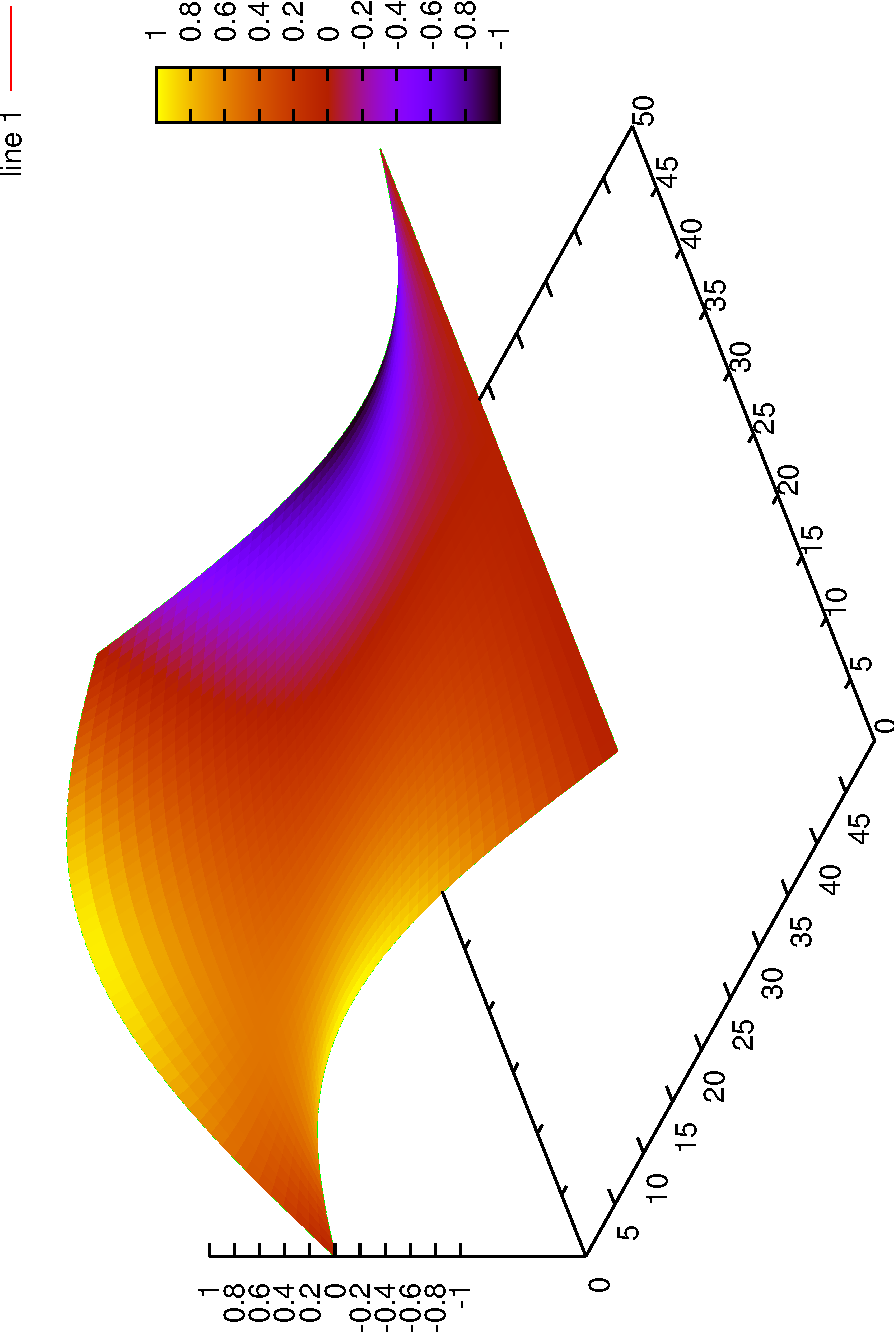
\includegraphics[%
  width=9cm,
  keepaspectratio,
  angle=-90]{figuras/mesh}


\caption{\label{cap:Superficie-soluci=F3n}Superficie solución}
\end{figure}


En el capítulo dedicado a la representación gráfica de soluciones
hemos hablado sobre lo poco útiles que suelen ser las superfícies
coloreadas para dar un resultado. Aunque una de estas representaciones
pueda parecer muy explicativa e intuitiva nunca debemos perder de
vista que lo que nos importa es mostrar un resultado y una superfície
no lo consigue. Por muy bien que coloquemos los colores o las barras
no conocemos el valor de cada punto con precisión y si encima colocamos
líneas de nivel dotamos al gráfico de un exceso de información.

Aunque sea mucho más espartano y pueda parecer inapropiado la solución
al problema son las curvas de nivel, en inglés \emph{contours} . Aunque
en un principio cueste un poco más entender la solución estamos ofreciendo
muchísima más información de un modo netamente más simple. Se podría
decir que no hay motivos para no utilizar las curvas de nivel a parte
de intentar demostrar nuestra pericia en el uso de Matlab.

%
\begin{figure}[H]
\centering{}

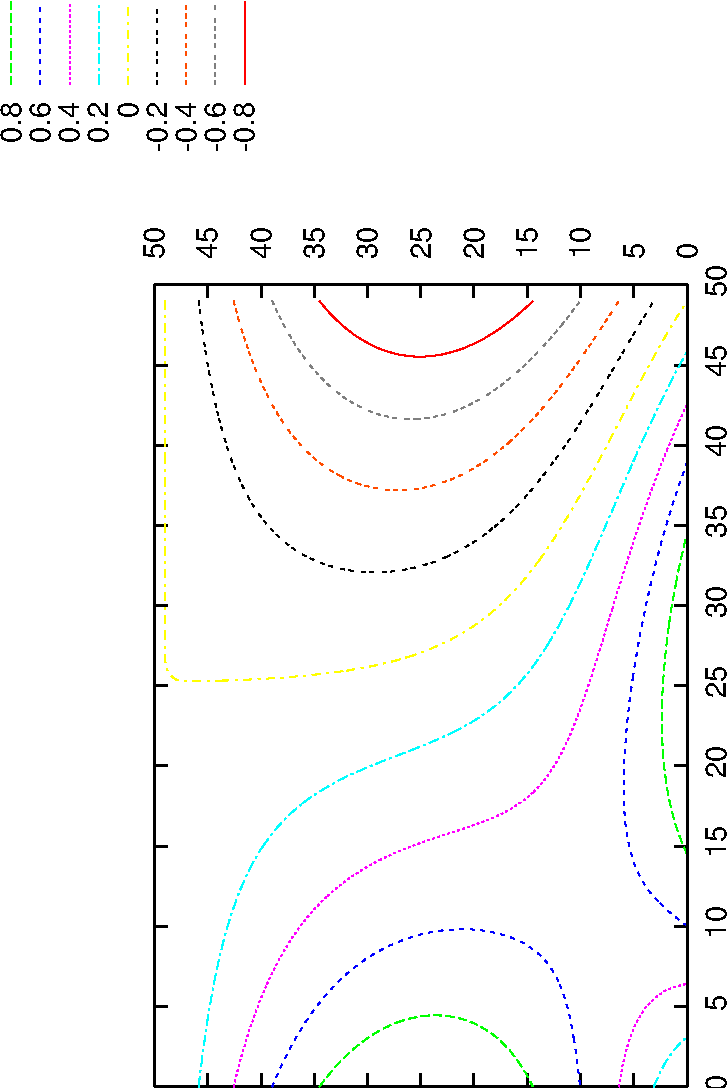
\includegraphics[%
  width=9cm,
  keepaspectratio,
  angle=-90]{figuras/contour}


\caption{\label{cap:Contorno-solucion}Superficie solución}
\end{figure}


Los gráficos de curvas de nivel pueden ajustarse perfectamente a nuestras
necesidades. Una práctica muy común y beneficiosa es la de embeber
el valor de cada curva dentro de la misma para no obligar al lector
a mirar la leyenda.


\subsubsection{Mejorar la solución. Cálculo de tiempos.}

Si analizamos el código de la solución es evidente que estamos
utilizando pocas funciones de la biblioteca. Además estamos haciendo
una de las pocas cosas casi prohibidas en Matlab que es crear una
matriz por fuerza bruta.

Un primer paso para mejorar la ejecución de un código es comprobar qué
partes consumen más recursos e intentar mejorarlas aisladamente.  Si
no somos capaces de conseguirlo nos replantearemos la solución de un
modo global. Para calcular los tiempos llenaremos el código con las
funciones \texttt{tic} y \texttt{toc}.

\begin{verbatim}
dx=2;
dy=3;
n=50;
m=50;
function place=place(i,j,n)
  place=i+n*(j-1);
end
A=zeros(n*m,n*m);
tic
for i=1:n*m
...
end
toc;disp('Creacion de la matriz del sistema'),disp(toc);tic;
i=1;
for j=1:m
  b(place(i,j,n))=sin(pi*(j-1)/(m-1));
...

  b(place(i,j,n))=0;
end
toc;disp('Creacion del vector b'),disp(toc);tic;
T=A \b';
toc;disp('Resolucion del sistema'),disp(toc);
T=reshape(T,n,m);
\end{verbatim}
Los tiempos en cada paso son:

\begin{verbatim}
>> ejercicio4
Creacion de la matriz del sistema
1.0611
Creacion del vector b
0.017038
Resolucion del sistema
2.1457
\end{verbatim}
Parece que debemos mejorar la construcción de la matriz del sistema y
la resolución del mismo. ¿Cómo? El primer paso suele ser analizar la
forma de la matriz con la función \texttt{spy}.

\begin{verbatim}
>> spy(A)
\end{verbatim}
Que tiene como resultado el siguiente patrón (figura
\ref{cap:Patr=F3n-de-elementos}):

%
\begin{figure}[h]
  \centering{}

  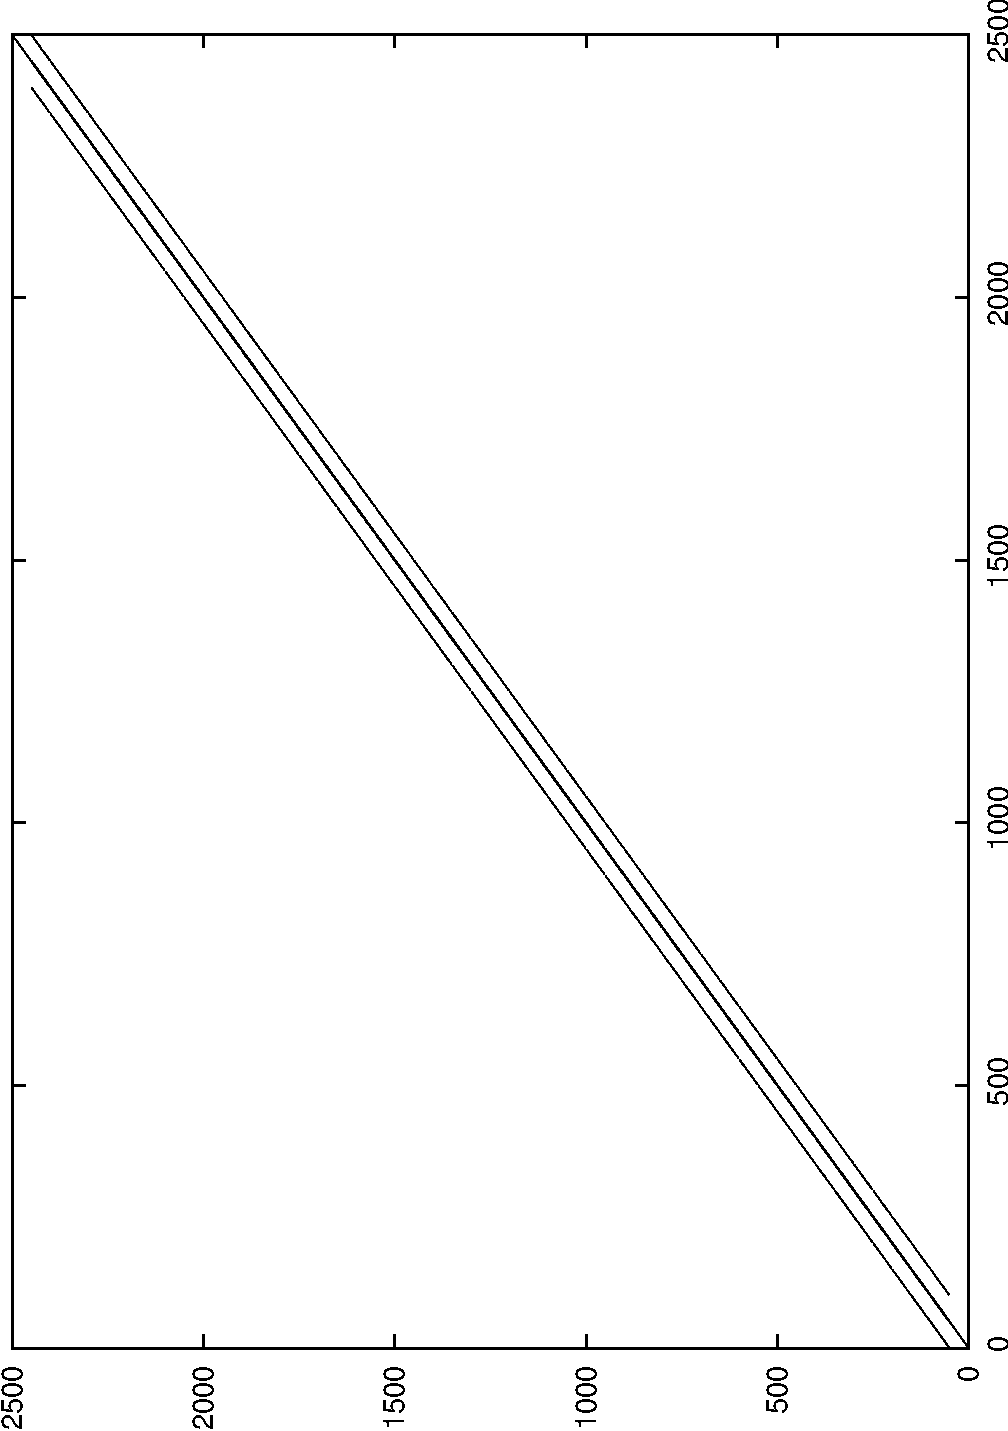
\includegraphics[%
  width=7cm,
  keepaspectratio,
  angle=-90]{figuras/spydiagonal}

  \caption{\label{cap:Patr=F3n-de-elementos}Patrón de elementos no
    nulos de la matriz del sistema}
\end{figure}


Esto nos demuestra que es una matriz n-diagonal por bandas lo que
entra en la definición de matriz sparse. Parece que la solución a
nuestros ligeros problemas de velocidad pueden solucionarse con el uso
de este tipo de matrices.


\subsubsection{Resolución del problema mediante matrices sparse(+)}

Uno de los errores cometidos en la primera solución propuesta es que
no utiliza las rutinas de creación de matrices disponibles. La
alternativa es utilizar bucles \texttt{for} para crearla por fuerza
bruta, solución de ningún modo recomendable. La mejor opción suele ser
utilizar la función \texttt{diag} pero como estamos tratando con
matrices sparse utilizaremos \texttt{spdiags}.


\subsubsection{Resolución del problema con un método iterativo.}

Para resolver el problema por un método directo es estrictamente
necesario romper la matriz para convertirla en un vector. Esto hace
que no podamos utilizar los operadores diferenciales en forma de
matriz tal como veremos en el ejercicio \ref{sec:Ejercicio-(Octave)}.
Un truco para mantener la integridad de la matriz y poder utilizar
estos operadores es resolver el problema con un método iterativo.
Aunque estemos multiplicando una matriz llena por matrices casi vacías
el resultado se acelera considerablemente.

La teoría de este método es bastante sencilla. Si aplicamos el
operador laplaciano a la matriz bidimensional el problema numérico se
reescribe del siguiente modo.$$
\mathbf{D_{x}}\phi+\phi\mathbf{D_{y}}^{\top}=0$$


Este planteamiento carece de solución analítica pero sirve para
plantear un problema iterativo en el que sólo hay que evaluar la
expresión.  Empezaremos la subrutina del mismo modo que la anterior,
definiendo la función que recoloca los elementos de la matriz
bidimensional.

\begin{verbatim}
dx=2;dy=3;global n=50;global m=50;
% resolucion del problema con un solver iterativo construccion de los
% operadores en diferencias
function place=place(i,j,n)
  place=i+n*(j-1);
end
\end{verbatim}
Ahora definiremos las matrices de los operadores diferenciales. Las
definimos como variables globales al igual que las dimensiones de la
matriz porque son necesarios dentro de la función que calcula el paso
de iteración y ésta puede tener sólo un argumento de entrada.

\begin{verbatim}
global DX=diag([1,-2/(dx*dx).*ones(1,n-2),1],0).+...
          diag([0,1/(dx*dx).*ones(1,n-2)],1).+...
          diag([1/(dx*dx).*ones(1,n-2),0],-1);
global DY=diag([1,-2/(dy*dy).*ones(1,n-2),1],0).+...
          diag([0,1/(dy*dy).*ones(1,n-2)],1).+...
          diag([1/(dy*dy).*ones(1,n-2),0],-1);
\end{verbatim}
A continuación la función que calcula el término en cada iteración.
Notemos el hecho de que el argumento que recibe la función debe ser un
vector por requerimientos de la rutina de resolución. Para calcular
sobre las matrices utilizamos la función \texttt{reshape}.

\begin{verbatim}
function [AT]=calcstuff(T)
  global n
  global m
  global DX
  global DY
  rT=reshape(T,n,m);
  AT=reshape((DX*rT)+(rT*DY'),n*m,1);
end
\end{verbatim}
Ahora es el turno del término independiente que se define gracias a la
función \texttt{place} definida anteriormente.

\begin{verbatim}
i=1;j=1;b=1;
for j=1:m
  b(place(i,j,n))=sin(pi*(j-1)/(m-1));
end
i=n;
for j=1:m
  b(place(i,j,n))=-sin(pi*(j-1)/(m-1));
end
j=1;
for i=1:n
  b(place(i,j,n))=sin(pi*(i-1)/(n-1));
end
j=n;
for i=1:n
  b(place(i,j,n))=0;
end
\end{verbatim}
Y finalmente resolvemos el sistema.

\begin{verbatim}
tic;T=pcg('calcstuff',b',tol=1e-6,maxit=100);
disp('Tiempo de calculo'),disp(toc)
\end{verbatim}
El método utilizado para resolver el problema es el del {}``Gradiente
Conjugado Precondicionado''. Para utilizarlo debemos tener en cuenta
que el número de iteraciones por defecto no es sufciente; lo
corregimos y lo situamos en 100. El tiempo de proceso ha pasado de más
de tres segundos a 0.24929%
\footnote{Este ejercicio se ha resuelto en un AMD Athlon 3000+.%
}. Este programa no sería posible sin el uso inteligente de las
variables globales tal como las hemos utilizado en otros ejemplos.


\section{\label{sec:Ejercicio-(Octave)}Ejercicio.  Un problema de
calor unidimensional}

\emph{Este ejercicio requiere la función} \texttt{\emph{trisolve}}
\emph{que está disponible en Octave. Matlab no tiene ninguna rutina
  para resolver directamente sistemas tridiagonales porque trata este
  tipo de matrices como sparse. Para resolver el mismo problema en
  Matlab utilizaremos la función} \texttt{\emph{spdiags}} \emph{para
  montar la matriz sparse y luego resolveremos el sistema de
  ecuaciones del modo usual.}

Este ejercicio es una pequeña demostración de hasta dónde puede llegar
el ahorro de código con Matlab. Se trata de resolver la ecuación del
calor unidimensional con condiciones de contorno Dirichlet. La
discretización espacial serán diferencias finitas de sevundo órden y
la temporal será un esquema Crank Nicholson. Tomaremos este esquema
porque permite usar saltos de tiempo más grandes, de hecho nos
permitirá llegar al resultado sin tener que calcular ninguna iteración
temporal. La solución propuesta tiene sólo unas pocas líneas.

Una solución tan breve requiere algo de preparación matemática de modo
que hay que estar muy atento al planteamiento analítico del problema.


\subsubsection*{Discretización de la ecuación completa}

La ecuación del calor unidimensional es la EDP parabólica más
sencilla:
$$\partial_{t}\phi=\partial_{xx}\phi$$
 Como cualquier EDP parabólica se
puede formular de la siguientes manera:
$$ \frac{d\phi}{dt}=F(x,t)$$ 
Si
utilizamos un esquema Crank Nicholson la discretización temporal será
de la forma:
$$ \frac{\phi^{n+1}-\phi^{n}}{\Delta
  t}=\frac{1}{2}\left(F^{n+1}+F^{n}\right)$$
 Discretizando también el
lado derecho de la ecuación con diferencias finitas de segundo orden
llegamos a la ecuación discretizada:$$ \phi_{i}^{n+1}-\frac{\Delta
  t}{2}\left(\frac{\phi_{i+1}^{n+1}-2\phi_{i}^{n+1}+\phi_{i-1}^{n+1}}{\Delta
    x^{2}}\right)=\phi_{i}^{n}+\frac{\Delta
  t}{2}\left(\frac{\phi_{n+1}^{n}-2\phi_{i}^{n}+\phi_{i-1}^{n}}{\Delta
    x^{2}}\right)$$



\subsubsection*{Formulación matricial del problema.}

La ecuación anterior puede escribirse del modo siguiente:\[
\phi^{n+1}-\frac{\Delta
  t}{2}\mathbf{A}\phi^{n+1}=\phi^{n}+\frac{\Delta
  t}{2}\mathbf{A}\phi^{n}\] Agrupando términos, diciendo que
$\mathbf{B}^{\pm}=\mathbf{I}\pm\frac{\Delta t}{2}\mathbf{A}$ y
utilizando un $\Delta x=1$ (en el fondo es sólo adimensionalizar):\[
\mathbf{B}^{-}\phi^{n+1}=\mathbf{B}^{+}\phi^{n}\] donde la matriz
$\mathbf{A}$ tiene la forma:\[ \mathbf{A}=\left(\begin{array}{cccccc}
    -2 & 1 & 0 & 0 & \cdots & 0\\
    1 & -2 & 1 & 0 &  & 0\\
    0 & 1 & -2 & 1 &  & 0\\
    \vdots &  &  & \ddots &  & \vdots\\
    0 &  & 0 & 1 & -2 & 1\\
    0 & \cdots & 0 & 0 & 1 & -2\end{array}\right)\]



\subsubsection*{Condiciones de contorno e iniciales.}

\begin{itemize}
\item Condiciones de contorno: $\phi=0$ en $x=0$ y $\phi=1$ en $x=10$ 
\item Condiciones iniciales: $\phi(x)=0$ en los puntos interiores.
\item Dar una solución al problema para cualquier tiempo inferior a $t=10$.
\end{itemize}

\subsection{Guía para la resolución del ejercicio}

La dificultad de la resolución de este problema radica en la correcta
situación de las condiciones de contorno en la matriz, el uso correcto
de las submatrices y entender el funcionamiento de \texttt{trisolve}.


\subsection{Solución del ejercicio (Octave)}

Parte del ejercicio es entender qué estamos haciendo para llegar a la
solución. Lo bueno de abreviar en la escritura es que además el código
resultante suele ser mucho más rápido.

\begin{verbatim}
phi=zeros(10,1); phi(10,1)=1;
dt=0.1;
for i=1:50 #Activate loop in case of precision leak
  phi(2:9)=(1-dt)*phi(2:9)+0.5*dt*phi(1:8)+0.5*dt*phi(3:10);
  phi=trisolve(-[0.5*dt*ones(8,1);0],[1;(1+dt)*ones(8,1);1],...
  -[0;0.5*dt*ones(8,1)],phi);
end
\end{verbatim}
De este modo llegamos al resultado del problema con una precisión
aceptable. La figura del perfil de temperaturas es:

%
\begin{figure}[H]
  \centering{} \includegraphics[width=14cm,
  keepaspectratio]{figuras/calor}

  \caption{\label{cap:figcalor}Figura solución}
\end{figure}



\subsection{Solución del ejercicio (Matlab)}

Aunque la resolución de sistemas tridiagonales es un clásico del
cálculo numérico Matlab no cuenta con ninguna función para ello. El
motivo es que decidieron incluir las matrices tridiagonales dentro de
las matrices sparse. Las matrices tridiagonales o con pocas bandas se
resuelven eficientemente mediante un método directo con lo que en este
caso Matlab tiene un error de diseño.

No tendría ningún sentido programarse una función que resolviera
sistemas tridiagonales en Matlab porque todas estas rutinas son en el
fondo interfaces a bibliotecas en Fortran y en C por motivos de
velocidad.

En este caso la dimensión de la matriz no justifica el uso del
almacenamiento sparse de modo que utilizaremos la función
\texttt{diag} para crear una matriz según sus diagonales:

\begin{verbatim}
phi=zeros(10,1); phi(10,1)=1; dt=0.1;
B=diag([1,(1+dt)*ones(1,8),1],0)+...
    diag(-[0.5*dt*ones(1,8),0],-1)+...
    diag(-[0,0.5*dt*ones(1,8)],1);
for i=1:50
  phi(2:9)=(1-dt)*phi(2:9)+0.5*dt*phi(1:8)+0.5*dt*phi(3:10);
  phi=B \phi;
end
\end{verbatim}

\subsection{Comprobación de la evolución temporal}

La siguiente modificación del programa permite comprobar la evolución
de los pasos temporales sacando por pantalla varios estados temporales
de la solución. Aunque el problema es estable para saltos temporales
muy grandes preferiremos acortarlo por motivos de precisión.
Representaremos la solución en los tiempos
$t=[0.1,1,2,5,10,20,50,100]$. Muy atentos al modo de definir la
condición lógica que indica cuándo pintar la curva:

\begin{verbatim}
phi=zeros(10,1); phi(10,1)=1;dt=0.1;
# times to output
tout=[0.1,1,2,5,10,20,50,100];
hold on
for i=1:500 
  phi(2:9)=(1-dt)*phi(2:9)+0.5*dt*phi(1:8)+0.5*dt*phi(3:10);
  phi=trisolve(-[0.5*dt*ones(8,1);0],[1;(1+dt)*ones(8,1);1],...
  -[0;0.5*dt*ones(8,1)],phi);
  if sum((dt*i)*ones(1,length(tout))==tout)==1
    plot(phi)
  end
end
hold off
title('Solucion de la ecuacion del calor unidimensional')
xlabel('Longitud (adimensional)')
ylabel('Temperatura (adimensional)')
legend({'0.1','1','2','5','10','20','50','100'},2)
\end{verbatim}
Llegamos finalmente a la siguiente gráfica:

%
\begin{figure}[H]
  \centering{} \includegraphics[width=14cm,
  keepaspectratio]{figuras/calorevol}


  \caption{Evolución del perfil de temperaturas}
\end{figure}


\section{Ejercicio.  Métodos espectrales.}
\subsection{Introducción}

Los métodos espectrales son útiles cuando se busca una gran precisión
en problemas de contorno. Por ejemplo, tomemos esta ecuación diferencial
no lineal\[
L(u)=u_{xx}-(x^{6}+3x^{2})u=0\]
con condiciones de contorno:\[
u(-1)=u(1)=1\]


¿Cómo podemos resolver esta ecuación diferencial? Podríamos utilizar
un esquema de diferencias finitas. Sería sencillo pero... ¿Quien ha
dicho que vamos a escoger el método más sencillo?

Uno de los objetivos de este ejercicio es realizar una breve introducción
práctica a los métodos espectrales de resolución de ecuaciones diferenciales.
Son más complicados y específicos pero más precisos y una herramienta
más potente en manos expertas.

Los métodos espectrales se basan en descomponer la solución en una
suma de funciones base que, multiplicadas por una serie de coeficientes,
aproxima la solución:\[
u_{N}=\sum_{i=0}^{N}a_{i}\phi_{i}(x)\]
Definimos el residuo como la diferencia entre la solución exacta y
la aproximada por nuestro desarrollo:\[
R(x;a_{i})=u(x)-u_{N}(x;a_{i})\]


Los métodos espectrales intentan reducir el residuo en lo posible.
Para ello se calcula\[
R(x;a_{i})=\partial_{xx}u_{N}-(x^{6}+3x^{2})u_{N}\]
e iguala el residuo a cero en determinados puntos del dominio. Esta
técnica se llama método \emph{Pseudoespectral} o de \emph{Colocación}.

Vamos a intentar resolver la ecuación anterior mediante un método
pseudoespectral utilizando una base de funciones del tipo:\[
u_{N}(x;a_{i})=1+(1-x^{2})(a_{0}+a_{1}x+a_{2}x^{2}+\cdots+a_{N}x^{N})\]


Si nos fijamos, la elección del desarrollo tiene bastante lógica.
Es un término constante acorde con las condiciones de contorno, una
función que asegura que las condiciones de contorno se cumplan siempre
y un desarrollo polinómico de potencias pares porque se deduce de
la ecuación que la solución será simétrica.

Con esta solución calcularemos el residuo y lo igualaremos a cero
en los puntos de Gauss-Chebyshev:\[
x_{i}=cos\left(\frac{(2i-1)\pi}{2N}\right)\]



\subsection{Algoritmo.}

Implementar el algoritmo no es tan difícil, lo que es más complicado
es encontrar la forma óptima de hacerlo en Matlab. Para ello nos crearemos
un vector de coeficientes \emph{$a=[a_{0},a_{1},a_{2},\ldots,a_{N}]^{T}$}
\emph{ordenado inversamente a como hace Matlab}. Entonces el polinomio
se calcularía con:\[
p(x)=\sum_{i}a_{i}x^{i}\]


Un método muy utilizado en estos casos es crear una serie de operadores
que actúan sobre los coeficientes. Estos operadores son distintos
para cada caso y se representan como una matriz que multiplicará nuestro
vector de coeficientes. Necesitamos los operadores $c\cdot$,$\partial_{xx}$,
$x^{6}$y $x^{2}$%
\footnote{Nótese que este algoritmo ignora la simetría puesto que tiene en cuenta
todos los coeficientes, tanto los pares como los impares.%
}.


\subsubsection{Operador $c\cdot$}

El operador de producto por un escalar aplicado a los coeficientes
de un polinomio es equivalente a:\[
c\cdot M=c\cdot M_{ij}\]
siendo $M$ una matriz cualquiera la matriz identidad.


\subsubsection{Operador $\partial_{xx}$}

Si tomamos un polinomio:\[
p(x)=a_{0}+a_{1}x+a_{2}x^{2}+a_{3}x^{3}+\cdots\]
y lo derivamos dos veces respecto a $x$ el resultado será:\[
\partial_{xx}p(x)=2\cdot1a_{2}+3\cdot2a_{3}x+4\cdot3a_{4}x^{2}+\cdots\]


El efecto sobre el vector de coeficientes $a$ será hacerlo pasar
de $a=[a_{0},a_{1},a_{2},a_{3},\ldots]^{T}$ a $\partial_{xx}a=[2\cdot1a_{2},3\cdot2a_{3},4\cdot3a_{4},\ldots]^{T}$.
La matriz que representa esta transformación tiene la forma:\[
\partial_{xx}=\left[\begin{array}{cccccccc}
0 & 0 & 2\cdot1 & 0 & 0 & 0 & \cdots & 0\\
0 & 0 & 0 & 3\cdot2 & 0 & 0 & \cdots & 0\\
0 & 0 & 0 & 0 & 4\cdot3 & 0 & \cdots & 0\\
0 & 0 & 0 & 0 & 0 & 5\cdot4 & \cdots & 0\\
\vdots & \vdots & \vdots & \vdots & \vdots & \vdots & \ddots & 0\\
0 & 0 & 0 & 0 & 0 & 0 & 0 & N(N-1)\end{array}\right]\]



\subsubsection{Los operadores $x^{6}$y $x^{2}$}

Cuando un polinomio\[
p(x)=a_{0}+a_{1}x+a_{2}x^{2}+a_{3}x^{3}+\cdots\]
es multiplicado por una potencia de su variable los coeficientes se
mueven hacia las potencias mayores tantas posiciones como sea la potencia
de la variable. La matriz será entonces, para el caso $x^{2}$:\[
x^{2}=\left[\begin{array}{cccc}
0 & 0 & 0 & \cdots\\
0 & 0 & 0\\
1 & 0 & 0\\
0 & 1 & 0\\
0 & 0 & 1\\
\vdots &  &  & \ddots\end{array}\right]\]


\lyxline{\normalsize}

Ejercicio1: Crear tres funciones que generen las matrices correspondientes
a los operadores $\partial_{xx}$(\emph{dxx.m}), y $x^{n}$(\emph{xn.m})
para un vector $a$ de $M$ elementos.

%
\framebox{\begin{minipage}[t][1\totalheight]{0.8\columnwidth}%
Debe tenerse en cuenta que $M=N+1$%
\end{minipage}}%


Solución:\emph{}\\
\emph{dxx.m}

\begin{lyxcode}
function~ret=dxx(M)



\%~~argumentos:

\%~~~~M~::~escalar~entero

\%~~Retorna~el~operador~derivada~segunda~para

\%~~un~vector~de~coeficientes~de~tamano~M



if~isscalar(M)

~~ret={[}zeros(M-2,1),zeros(M-2,1),diag(2:M-1).{*}diag(1:M-2)];

else

~~disp('M~debe~ser~un~escalar')

end
\end{lyxcode}
\emph{xn.m}

\begin{lyxcode}
function~ret=xn(M,n)



\%~~argumentos:

\%~~~~M~::~escalar~entero

\%~~~~n~::~escalar~entero

\%~~Retorna~la~matriz~correspondiente~al~operador

\%~~x\textasciicircum{}n~con~n~cualquier~exponente~entero~para~un

\%~~vector~de~coeficientes~de~M~elementos



if~isscalar(M)~\&\&~isscalar(n)

~~ret={[}zeros(n,M);eye(M)];

else

~~disp~('Ambos~argumentos~deben~ser~escalares')

end
\end{lyxcode}
\lyxline{\normalsize}


\subsubsection{El operador Residuo.}

Es evidente que los tres operadores anteriores son lineales respecto
al vector de coeficientes $a$, entonces el operador suma y la multiplicación
por un escalar van a tener los mismos efectos que en la \emph{realidad:}\[
R(a)=\partial_{xx}(a)-x^{6}(a)-3x^{2}(a)\]
van a ser los coeficientes del polinomio del residuo.

Pero aún no hemos construido nuestro operador Residuo. Este es el
operador aplicado a un polinomio de la forma usual. Nuestro desarrollo
en funciones base es ligeramente distinto:\[
a'=(1-x^{2})a\]
Llamaremos a este operador $b$.

\lyxline{\normalsize}

Ejercicio 2: A partir de las funciones anteriores construir el operador
$b$ para un vector $a$ de $M$ elementos.

La solución a este ejercicio plantea el siguiente problema: Si intentamos
utilizar la función cdot juntándola con la función \emph{xn} con n=2
aparece el inconveniente de que las matrices no son compatibles. Como
este problema se va a repetir más adelante crearemos una función que
adapte las matrices y les añada tantos ceros como sea necesario para
hacerlas compatibles con la matriz mayor. Esta función se llamará
\emph{join}

Solución:\\
\emph{join.m}

\begin{lyxcode}
function~ret=join(A,B)



\%~~argumentos:

\%~~A~::~Matriz,~real

\%~~B~::~Matriz,~real

\%~~Devuelve~una~copia~de~la~matriz~A~compatible

\%~~con~la~matriz~B~en~el~caso~que~sean~transformaciones

\%~~de~un~vector



sizA~=~size(A);

sizB~=~size(B);

if~sizA(2)~==~sizB(2)~\&\&~sizA(1)~<~sizB(1)

~~ret={[}A;zeros(sizB(1)-sizA(1),sizA(2))];

else

~~disp('Las~matrices~no~son~compatibles')

~~ret=0;

end
\end{lyxcode}
\emph{Creación de la matriz b en función de M:}

\begin{lyxcode}
function~ret=b(M)

\%~~argumentos:

\%~~M~::~escalar~entero

x2~=~xn(M,2);

ret~=~join(eye(M),x2)-x2;
\end{lyxcode}
\lyxline{\normalsize}

Para por fin construir el operador residuo utilizaremos la composición
de aplicaciones lineales, es decir, el producto matricial:

\[
R(a')=\partial_{xx}(a')-x^{6}(a')-3x^{2}(a')\]
\[
R(a')=(\partial_{xx}\cdot b)(a)-(x^{6}\cdot b)(a)-(3x^{2}\cdot b)(a)\]
\[
R(a')=\left[(\partial_{xx}\cdot b)-(x^{6}\cdot b)-(3x^{2}\cdot b)\right](a)\]


\lyxline{\normalsize}

Ejercicio 3: Crear a partir de los operadores anteriores la función
que genere el operador $R$ en función de $M$ teniendo en cuenta
que los resultados parciales pueden generar vectores de tamaños distintos.
Esto significa que se va a reproducir el problema que ya encontramos
en el segundo ejercicio pero esta vez no existe una solución universal.

Solución:\\
R.m

\begin{lyxcode}
function~ret=R(M)

\%~Dificil~de~descifrar.~~Comentario~pendiente

\%~Fuciona.

dxxb~=~dxx(M+2){*}b(M);\%~Primer~termino

x6b~=~xn(M+2,6){*}b(M);\%~Segundo~termino

x2\_3b~=~3{*}xn(M+2,2){*}b(M);\%~Tercer~termino

ret~=~join(dxxb,x6b)-x6b-join(x2\_3b,x6b);
\end{lyxcode}
\lyxline{\normalsize}

Definimos $a''$ como $a''=R(a)$, o en forma matricial: $a''=R\cdot a$


\paragraph{Retener los términos independientes:}

Alguien especialmente observador habrá notado que en el operador $b$
parece que falta un término, un $+1$. Se ha eliminado de los operadores
porque al no ser dependiente de ningún coeficiente queda como término
independiente. Este término debe calcularse a parte%
\footnote{Parte de la tarea de la elección de buenas funciones base está en
evitar que aparezcan estos términos independientes.%
}.

Si pasamos este $+1$ por el operador $L$ obtenemos que el término
independiente es $x^{6}+3x^{2}$.


\subsubsection{Sistema de ecuaciones.}

Ahora nos falta igualar el residuo en los puntos de Gauss-Chebyshev
a cero. Esto da tantas ecuaciones del tipo $R(x,a_{i})$ como sean
necesarias. Llamando a un punto en concreto $\xi_{i}$ cada ecuación
tendrá la forma:\[
a_{0}^{\prime\prime}+a_{1}^{\prime\prime}\xi_{i}+a_{2}^{\prime\prime}\xi_{i}^{2}+a_{3}^{\prime\prime}\xi_{i}^{3}+\cdots=\xi_{i}^{6}+3\xi^{2}\]
llamamos entonces al sistema:\[
Sa''=q\]


\lyxline{\normalsize}

Ejercicio 4: Plantear un sistema de ecuaciones anterior para los puntos:\[
\xi_{i}=cos\left(\frac{(2i-1)\pi}{2M}\right)\]


Recordad que el vector $a''$ es de dimensiones diferentes a $a$.
En el caso que nos ocupa el número de elementos de $a''$ es mayor
al de $a$. Como el sistema que intentamos resolver en realidad es:\[
(SR)a=q\]
la matriz del sistema $S$ debe ser compatible con el operador Residuo
$R$. Para ello, el número de ecuaciones, el número de filas de $M$,
debe ser igual al número de elementos de $a$.

Solución:\\
\emph{SRq.m}

\begin{lyxcode}
function~{[}S,q]=SRq(R)

\%~~calcula~la~matriz~SR~en~funcion~de~la~matriz~residuo~R

\%~Nodos~de~Gauss~Chebyshev

\%~Tomo~M~de~R

M=size(R)(2);~\%esto~es~legal~en~Octave~pero~ilegal~en~Matlab

~~~~~~~~~~~~~~\%Octave~permite~una~escritura~mucho~mas~compacta

ngc=(cos((2{*}(1:M)-1){*}pi/(2{*}M))).';

grado=size(R)(1);

\%No~hay~mas~remedio~que~utilizar~un~bucle.

S=R';

for~i=0:grado-1

~~S(:,i+1)=ngc.\textasciicircum{}i;

end

q=ngc.\textasciicircum{}6+3{*}ngc.\textasciicircum{}2;
\end{lyxcode}
\lyxline{\normalsize}

Ahora sólo nos falta resolver el sistema de ecuaciones final:\[
(S\cdot R)a=q\]
siendo q el vector de términos independientes que hemos calculado
a parte.

\lyxline{\normalsize}

Ejercicio 5: Resolver el sistema de ecuaciones para calcular $a$
para $M$=5, 10, 20 y 30. Como todo está en función de $M$ no debería
haber ningún problema.

Solución:

\begin{lyxcode}
r=R(5);

{[}s,q]=SRq(r);

solM5=(s{*}r)\textbackslash{}q;



r=R(10);

{[}s,q]=SRq(r);

solM10=(s{*}r)\textbackslash{}q;



r=R(20);

{[}s,q]=SRq(r);

solM20=(s{*}r)\textbackslash{}q;



r=R(30);

{[}s,q]=SRq(r);

solM30=(s{*}r)\textbackslash{}q;
\end{lyxcode}
\lyxline{\normalsize}


\subsection{Análisis de los resultados.}

La solución analítica del problema es {[}Scraton, 1965]:\[
u(x)=exp\left(\frac{x^{4}-1}{4}\right)\]
Esto nos permite comparar el resultado obtenido con la solución, algo
que será imposible hacer en la mayoría de los problemas no lineales.

\lyxline{\normalsize}

Ejercicio 6: Representar gráficamente la solución analítica junto
con cada una de las soluciones obtenidas anteriormente. Debemos tener
en cuenta que los coeficientes que hemos obtenido en el ejercicio
anterior no son de un polinomio Matlab por dos motivos:

\begin{enumerate}
\item Están almacenados en el orden inverso
\item El desarrollo polinómico real es de la forma:
\end{enumerate}
\[
u_{N}(x;a_{i})=1+(1-x^{2})(a_{0}+a_{1}x^{1}+a_{2}x^{2}+\cdots+a_{N}x^{N})\]
Para transformar los coeficientes en el polinomio solución crearemos
una función llamada \emph{transsol} que nos devolverá el polinomio
solución.

Solución:\\
transsol.m

\begin{lyxcode}
function~ret=transsol(sol)

\%~~argumentos

\%~~~~sol~::~vector~real

\%~~~~~~~~~~~vector~de~coeficientes~solucion~del~problema

sol=rot90(rot90(sol));

sol=conv({[}-1,0,1],sol);

sol(length(sol))++;~\%~Operador~sólo~válido~en~Octave

ret=sol;~~~~~~~~~~~~~~~~~~~~\%~proviene~de~C
\end{lyxcode}
Ahora, para representar gráficamente las soluciones:

\begin{lyxcode}
>\,{}>~x~=~linspace(-1,1,100);

>\,{}>~plot(x,exp((x.\textasciicircum{}4-1)/4));

>\,{}>~hold~on

>\,{}>~plot(x,polyval(transsol(solM5),x));

>\,{}>~plot(x,polyval(transsol(solM10),x));

>\,{}>~plot(x,polyval(transsol(solM20),x));

>\,{}>~plot(x,polyval(transsol(solM30),x));
\end{lyxcode}
La precisión del resultado es tan alta que no se distinguen las curvas
a partir de $M=10$.

\begin{center}
\includegraphics{figuras/ejercicio_espectral_scripts/solucion}

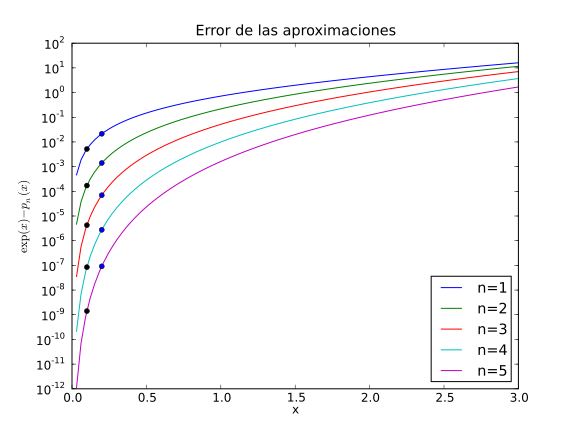
\includegraphics{figuras/ejercicio_espectral_scripts/error}
\end{center}

\lyxline{\normalsize}


\subsubsection{Convergencia.}

En la mayoría de los casos es imposible saber si la solución que obtenemos
es la real, lo que sí podemos analizar es si nuestro algoritmo converge
a una determinada solución. La convergencia de los métodos espectrales
es, como ya hemos visto, especialmente buena.

Para asegurarnos que la solución converge debemos demostrar que entre
los términos que obviamos (las potencias mayores) no son lo suficientemente
relevantes como para influir en la solución. Un gráfico especialmente
útil es el que representa el logaritmo del módulo de los coeficientes
en función del número de término que representan.

Calcularemos tomaremos el caso $M=30$ y representaremos $log|a_{n}|$en
función de $n$.
\begin{center}
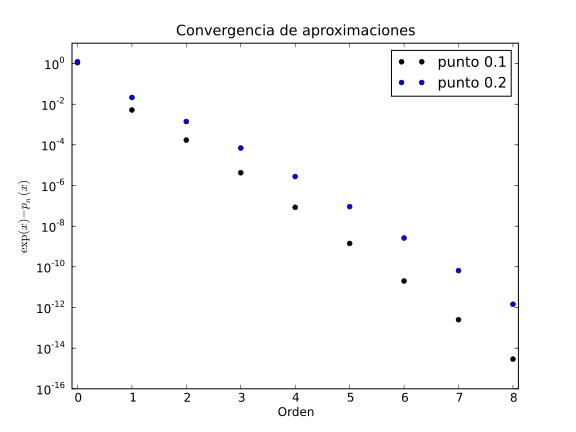
\includegraphics{figuras/ejercicio_espectral_scripts/convergencia}
\end{center}

Si se toma la tendencia de los coeficientes el problema converge hacia
una solución. Lo más sorprendente es que, como la solución es simétrica,
los coeficientes impares deberían ser nulos.El mayor coeficiente impar
tiene un valor máximo equivalente al $\epsilon$del real de doble
precisión lo que nos induce a pensar que el error es debido a la precisión
numérica del método utilizado.


\subsection{Análisis crítico}

Las soluciones del ejercicio anterior no son perfectas, de hecho,
podrían ser bastante mejores. Se han introducido ciertos errores de
estilo a drede para poder analizarlos con más detenimiento.

Un pequeño error es el hecho de utilizar condicionales para los errores
en las dimensiones de las matrices. Si dos argumentos son incompatibles
en una operación octave tiene todo un sistema de errores dedicado
a ello, generar errores no estándar puede confundir al usuario al
dar información redundante. Desde el punto de vista de código tolerante
a fallos es más interesante una estructura tipo try-catch o una unwind\_protect
en octave.

Otro pequeño error es utilizar estructuras en octave que no sean portables.
Desde el punto de vista de un programador experimentado parece siempre
una buena idea utilizar todo lo que el lenguaje de programación puede
ofrecer pero este es un caso especial. No es razonable pasar un script
a alguien pensando que será capaz de resolver la incompatibilidad.

El problema de las incompatibilidades entre Matlab y Octave es muy
grave, no porque sean muy distintos sino porque sus diferencias son
sutilezas. En algunos casos Octave corrige inconsistencias de Matlab
o añade posibilidades. En otros casos es Matlab el que dispone de
una función perfecta para una tarea pero no Octave. Escribir código
portable entre los dos intérpretes no es difícil pero requiere haberse
leído detenidamente el FAQ del proyecto Octave

